\documentclass[]{auvsi_doc}
\setkeys{auvsi_doc.cls}{
	AUVSITitle={Airframe Concept Description},
	AUVSILogoPath={./figs/logo.pdf}
}

% include extra packages, if needed

\begin{document}

\begin{AUVSITitlePage}
\begin{artifacttable}
\entry{AF-002, 0.1, 10-31-18, Initial Draft, Tyler Critchfield, Ryan Anderson}
% additional \entry{} commands for extra rows in the revision table, if needed
\end{artifacttable}
\end{AUVSITitlePage}

\section{Introduction}

The purpose of this subsystem concept selection process was to select an airframe concept that would allow the UAS to complete its mission with the highest number of points possible, including flying slower and with an increased capacity to fit our UGV payload. This artifact describes our chosen concept.

\section{Concept Description}

We selected the modified Nimbus Pro as our chosen concept for the Airframe subsystem. This airframe modifies a traditional twin propulsion fixed wing RC airframe (see Figure \ref{fig:nimbus}) that can be purchased off the shelf. The original RC airframe has a wing span of 1.95m, a wing area of 5700 cm$^2$, a fuselage length of 1.29m, a payload storage volume of about 8000 cm$^3$, and an empty weight of 1.9 kg. In this design, about two-thirds of the wings are able to be disconnected for easy storage and transport (see Figure \ref{fig:wing}). We could use this to our advantage and create new wing extensions to attach to the plane instead of the original wings. These wing extensions would likely have a longer span, but would be restricted to the existing design in root airfoil shape and root chord length. We would have freedom to adjust span, taper ratio, tip twist, and a tip airfoil if we choose to. We would model these design parameters in XFLR5 to determine the best wing extension design. The wing extensions would be made of foam and easily constructed using the foam cutter in the EB lab. The modular nature of these adjustments would make it easy to assemble and rebuild if necessary, especially if redundant parts are purchased and created. This is critical to our team's success this year. To be successful, each subsystem will need to prototype and test their designs often - but no one can truly test their designs without an airframe that flies. Having a modular wing design would still allow for fast rebuild, ensuring that other team members would not be wasting time waiting for a new plane to be built. In the case that a redesign is necessary, the other subsystem teams can use the existing wings for the Nimbus Pro while waiting.

\begin{figure}[h!]
	\centering
	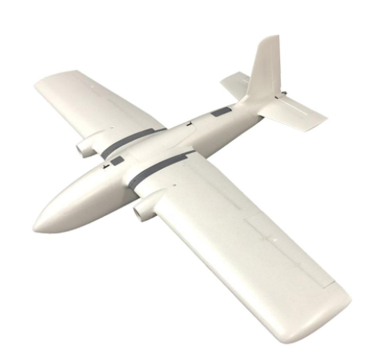
\includegraphics[scale=0.7]{figs/NimbusPro}
	\caption{The Nimbus Pro from My Fly Dream. Image taken from banggood.com.}
	\label{fig:nimbus}    
\end{figure}

\begin{figure}[h!]
	\centering
	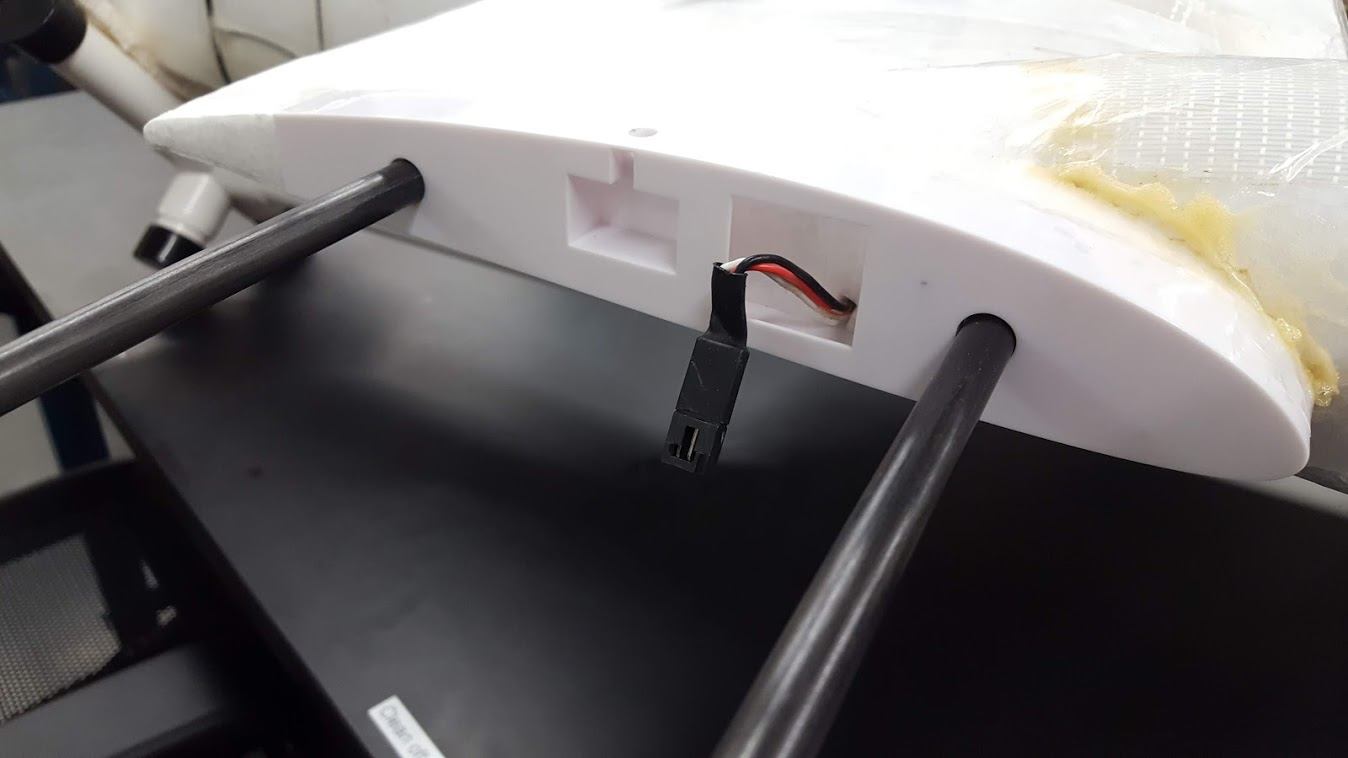
\includegraphics[width=.8\columnwidth]{figs/wing}
	\caption{This is where the wing dissassembles and where we would attach our custom wings. This is a photo of My Twin Dream, but this concept is the same for the Nimbus Pro.}
	\label{fig:wing}    
\end{figure}

\end{document}